\chapter{Integración con un recomendador externo}

En este capítulo se mostrará como se realiza la integración con un recomendador externo mediante un sistema bidireccional dirigido por eventos y el intercambio de mensajes JSON.

\section{Introducción}

Tal y como hemos mencionado anteriormente el simulador y el recomendador están integrados mediante un sistema bidireccional dirigido por eventos y el intercambio de mensajes en JSON. Actualmente está desarrollado un recomendador de ejemplo basado en usuarios de tipo pull mediante la librería Apache Mahout. 

La razón por la que se han integrado los dos sistemas mediante un sistema bidireccional dirigido por eventos es que existen recomendadores que realizan recomendaciones sin que el usuario las haya solicitado. En protocolos como el HTTP no podemos enviar respuesta al navegador sin que este haya lanzado un petición previamente mientras que en el sistema bidireccional dirigido por evento si que podemos enviar datos al cliente cuando sea necesario y sin que este los haya solicitado. 

El recomendador de ejemplo desarrollado está pensado en lanzar un hilo para cada tipo de recomendador, es decir, un hilo para el servidor de tipo pull y otro para el recomendador de tipo push. Actualmente solo existe una implementación de un recomendador de tipo pull y por lo tanto solo hay un hilo. Este recomendador incorpora un patrón de diseño de tipo Strategy combinado con un patrón de diseño de tipo Factory que nos permiten cambar el tipo de implementación del recomendador de tipo pull en tiempo de ejecución. 

De esta manera podemos cambiar la implementación del recomendador de tipo pull entre peticiones y dar servicio a los distintos recomendadores configurados en las distintas escenas. 

A continuación se mostrará cual es el modelo de eventos para cada tipo de recomendador y cual es el forma de los mensajes intercambiados. 

\section{Recomendadores pull}

En está sección se mostrará la arquitectura del recomendador pull existente y como expandirlo para crear una nueva implementación para este tipo tipo de recomendador. 

\subsection{¿En que consiste el patrón de diseño de tipo Strategy?}

El patrón Strategy es un patrón de comportamiento porque determina cómo se debe realizar el intercambio de mensajes entre diferentes objetos para resolver una tarea. Permite mantener un conjunto de algoritmos de entre los cuales el cliente puede elegir cual le conviene usar. Tiene los siguiente participantes:

\begin{itemize}
	\item Contexto: es el elemento que usa los algoritmos y delega en la jerarquía de estrategias. Configura una estrategia mediante una referencia a la estrategia concreta.  
	\item Estrategia: una interfaz común para todos los algoritmos. Es usada por el contexto para invocar la estrategia concreta.
	\item Estrategia concreta: implementa el algoritmo utilizando la interfaz definida por la estrategia.
\end{itemize}

En nuestro caso el contexto es el objeto Recommender ubicado en el paquete recommender.context, la interfaz estrategia se corresponde la interfaz Strategy ubicada en el paquete recommender.strategy y la estrategia concreta es la clase UserBasedStrategy ubicada el paquete recommender.strategy. 

En la implementación actual se ha usado en patrón de diseño de tipo Factory para crear y gestionar las instancias de las estrategias concretas. Cuando llega una solicitud de recomendación por un usuario se crea una instancia de la estrategia concreta y se almacena en una tabla hash. Si la estrategia concreta ya este almacenada en la tabla hash entonces solo se devuelve la instancia de esta.

\subsection{Pasos para crear un nuevo recomendador pull}

\subsubsection{Paso 1: Crear una estrategia concreta}

Tal y como hemos mencionado anteriormente la estrategia concreta implementa el algoritmo de recomendación concreto. Para implementar un nuevo tipo de algoritmo de recomendación tenemos que crear una clase en el paquete recommender.strategy que implemente la interfaz Strategy del mismo paquete. 

Esta interfaz tiene dos métodos: recommend e itemForecast. El método recommend es el que se invoca cuando el usuario solicita una recomendación y devuelve una lista de ítems. El método itemForecast realiza una predicción para un ítem dado un usuario y devuelve un float que se corresponde a la predicción realizada.

Los parámetros de entrada de ambos métodos son iguales y tienen el mismo significado:

\begin{itemize}
	\item JSONObject data: contiene todos los datos en formato JSON que enviar el simulador.
	\item List$<$Item$>$ itemList: contiene un array list con todos los ítems a recomendar.
	\item List$<$Ratings$>$ ratingList: contiene un array list con las valoraciones de los usuarios para cada ítem.
	\item RecommenderConfig recommenderConfig: contiene los parámetros de configuración del recomendador como numero de ítems a recomendar etc.
\end{itemize}

Todos los datos vienen listos para ser usados por el algoritmo de recomendación que estamos implementando.

\newpage

\subsubsection{Paso 2: expandir el enumerado StrategyType}

StrategyType es un tipo enumerado que contiene todas las estrategias concretas implementadas. Es utilizado por patrón Factory para determinar que tipo de estrategia concreta crear. 

\begin{lstlisting}[language=xml, frame=single]
package recommender.models;

public enum StrategyType {
	UserBasedStrategy("User based recommender");
	
	private String type;
	
	StrategyType(String type) {
		this.type = type;  
	}
	
	public String getType() {
		return this.type;
	}

	public static StrategyType fromString(String type) {
		if (type != null) {
			for (StrategyType b : StrategyType.values()) {
				if (type.equalsIgnoreCase(b.type)) {
					return b;
				}
			}
		}
	
		return null;
	}
}
\end{lstlisting}

En la implementación de la figura anterior podemos ver el siguiente enumerado UserBasedStrategy($"$User based recommender$"$) que se corresponde a la implementación actual del algoritmo de recomendaciones basados en usuarios. La cadena entre comillas es el nombre que se va mostrar en el simulador cuando configuramos un nuevo recomendador.

\subsubsection{Paso 3: expandir el factory StrategyFactory}

Una vez que hayamos expandido StrategyType vamos a expandir el factory StrategyFactory para que pueda usar este nuevo tipo de enumerado y crear la estrategia concreta.

\begin{lstlisting}[language=java, frame=single]
package recommender.strategy;

import java.util.HashMap;
import java.util.Map;
import recommender.models.StrategyType;

public class StrategyFactory {
	static Map<StrategyType, Strategy> map = new HashMap<StrategyType, Strategy>();
	
	public static Strategy createStrategy(StrategyType type){
		Strategy strategy = map.get(type);
		
		if(strategy==null){
			switch(type){
			case UserBasedStrategy: strategy = new UserBasedStrategy(); break;
			default: throw new IllegalArgumentException("The recommender type " + type + " is not recognized.");
			}
			
			map.put(type, strategy);
		}
		
		return strategy;
	}
}
\end{lstlisting}

Para expandirlo vamos al método createStrategy y expandimos el switch para que use el nuevo enumerado que hemos creado en el paso 2 y en función a ellos cree una nueva instancia de la estrategia concreta que hemos creado en el paso 1. 

\subsection{Eventos y mensajes}

En el diagrama siguiente podemos ver cuales son todos los eventos en el recomendador de tipo pull:

\begin{figure}[H]
	\centering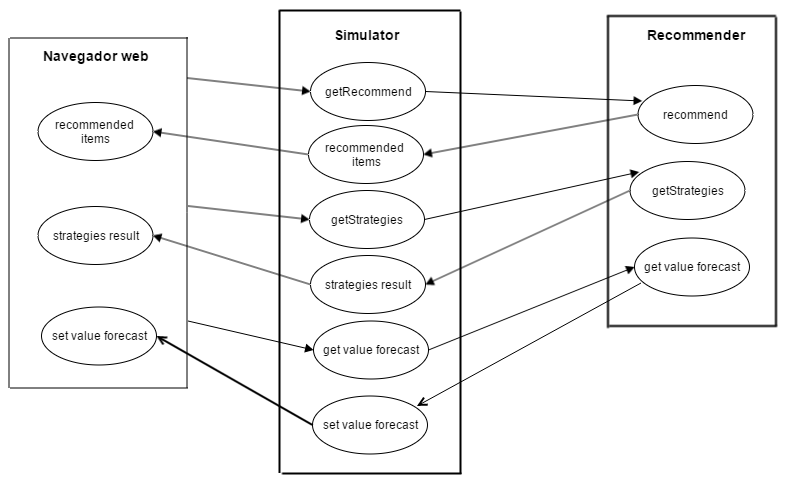
\includegraphics[scale=0.5]{imagenes/diagrama-de-eventos.png}
	\caption{Diagrama de eventos del recomendador de tipo pull}
	\label{img:diagramaEventosPull}
\end{figure}

Los eventos importantes del recomendador son:

\begin{itemize}
	\item recommend: es el evento que invoca el simulador para solicitar una recomendación.
	\item getStrategies: es el evento que se invoca para recuperar la lista de estrategias concretas implementadas. No tiene parámetros de entrada.
	\item get value forecast: es el evento que se invoca para solicitar una predicción para un ítem
\end{itemize}

Los eventos importantes del simulador son:
\begin{itemize}
	\item recommended items: es el evento que invoca el recomendador para enviar la lista de ítems recomendados.
	\item strategies result: es el evento que invoca el recomendador para enviar la lista de estrategias concretas implementadas.
	\item set value forecast: es el evento que invoca el recomendador para enviar la predicción para un ítem.
\end{itemize}

A continuación podemos ver los parámetros de entrada de los eventos importantes para una integración con un recomendador externo:

\begin{table}[H]
	\centering
	\label{my-label}
	\begin{tabular}{|l|l|p{7cm}|}
		\hline
		\multicolumn{1}{|c|}{\textbf{Nombre}} & \multicolumn{1}{c|}{\textbf{Tipo}} & \multicolumn{1}{c|}{\textbf{Descripción}}                                                                                   \\ \hline
		userId                                & String                             & token del usuario                                                                                                           \\ \hline
		strategyType                          & String                             & tipo de estrategia concreta que queremos usar para la recomendación. Contiene uno de los valores del enumerado StrategyType \\ \hline
		mapId                                 & String                             & identificador del mapa                                                                                                      \\ \hline
		sceneId                               & String                             & identificador de la escena                                                                                                  \\ \hline
		rating                                & number                             & Valoración del usuario sobre ítem con identificador itemId                                                                  \\ \hline
		itemId                                & String                             & identificador del item                                                                                                      \\ \hline
		recommenderId                         & String                             & identificador de la configuración del recomendador                                                                          \\ \hline
	\end{tabular}
	\caption{Evento get value forecast del recomendador}
\end{table}

\begin{table}[H]
	\centering
	\label{my-label}
	\begin{tabular}{|l|l|l|}
		\hline
		\multicolumn{1}{|c|}{\textbf{Nombre}} & \multicolumn{1}{c|}{\textbf{Tipo}} & \multicolumn{1}{c|}{\textbf{Descripción}}                    \\ \hline
		itemList                              & Array                              & lista con ítems que recomendamos al usuario                  \\ \hline
		userList                              & Array                              & lista de tokens de usuarios a los que recomendamos los items \\ \hline
	\end{tabular}
	\caption{Evento recommended ítems del simulador}
\end{table}

\begin{table}[H]
	\centering
	\label{my-label}
	\begin{tabular}{|l|l|p{6cm}|}
		\hline
		\multicolumn{1}{|c|}{\textbf{Nombre}} & \multicolumn{1}{c|}{\textbf{Tipo}} & \multicolumn{1}{c|}{\textbf{Descripción}}                                                                                                                                                                                                                                                                                                               \\ \hline
		strategyType                          & String                             & tipo de estrategia concreta que queremos usar para la recomendación. Contiene uno de los valores del enumerado StrategyType                                                                                                                                                                                                                             \\ \hline
		mapId                                 & String                             & identificador del map en el que está conectado el usuario                                                                                                                                                                                                                                                                                               \\ \hline
		sceneId                               & String                             & identificador de la escena en la que está conectado el usuario                                                                                                                                                                                                                                                                                          \\ \hline
		token                                 & String                             & token del usuario conectado                                                                                                                                                                                                                                                                                                                             \\ \hline
		recommender                           & String                             & identificador de la configuración del recomendador que estamos usando                                                                                                                                                                                                                                                                                   \\ \hline
		itemTypesToRecommend                  & Array                              & contiene una lista con los identificadores de los tipos de ítems sobre los que el usuario desea recibir recomendaciones                                                                                                                                                                                                                                 \\ \hline
		resultTypeShow                        & String                             & el tipo de resultado que quiere ver el usuario. Puede contener los siguiente valores: \newline - nonPersonalizedRecommendation: para mostrar recomendaciones no personalizadas en caso que de que el recomendador no tiene ítems que recomendar \newline - emptyList: para mostrar una lista vacia cuando el recomendador no tiene ítems que recomendar \\ \hline
		location                              & Object                             & localización actual del usuario. Es un objeto que contiene los siguientes atributos: \newline- longitude: longitud actual \newline - latitude: latitud actual                                                                                                                                                                                           \\ \hline
	\end{tabular}
	\caption{Evento recommend del recomendador}
\end{table}

\newpage

\section{Recomendadores push}

Para crear un recomendador de tipo push tenemos que editar el objeto Server y lanzar un nuevo hilo que se corresponde al recomendador de tipo push y pasarle en el constructor los parámetros configs y socket igual que el PullServer en el siguiente ejemplo: 

\begin{lstlisting}[language=java, frame=single]
public Server() throws URISyntaxException, InterruptedException, IOException{
	try {
		Configurations configs = readBaseConfig();
		String url = configs.getHost()+":"+configs.getPort();
		
		socket = IO.socket(url);
		socket.connect();
		
		//Inicializamos un servidor de tipo pull
		PullServer pullServer = new PullServer(configs, socket);
		pullServer.run();
	} catch (URISyntaxException e) {
		System.out.println(e);
	}
}
\end{lstlisting}

La variable config contiene datos a cerca de la dirección de la base de datos y la dirección del simulador. La variable socket es el sistema bidireccional dirigido por eventos. 

En cuanto a la arquitectura tenemos total liberar para el diseño del recomendador push. Lo único es que tenemos que hacer es crear el evento get strategies push. Este evento no tiene parámetros de entrada y devuelve una lista de enumerados con las implementaciones del recomendador push (ver implementación de la clase StrategyType). Para devolver la lista de recomendaciones tenemos que invocar el evento get strategies push result.

Para enviar las recomendaciones tenemos que usar el evento recommended items del simulador indicando la lista de ítems que estamos recomendado y la lista de usuarios (tokens) a los que realizamos las recomendaciones.
